\errorcontextlines=9999
\documentclass[
   aspectratio=169, % default is 43
   10pt, % font size, default is 11pt
   % nosectionframes,
   uniqueslidenumber,
   % handout,
   professionalfonts
]{beamer}

\usepackage[T1]{fontenc}
\usepackage[utf8]{inputenc}
\usepackage[sfdefault]{FiraSans}

\usepackage{stmaryrd}
\usepackage[vvarbb]{notomath}
\usepackage{FiraMono}
\usepackage{tikz,forest}
\usepackage{fontawesome}
\usepackage{csquotes}
\usepackage{simplebnf}
\usepackage{../abstract-interpretation-ltx/absint}
\makeatletter
\def\absint@reflab#1#2{#2}% we do not need labels here
\usetikzlibrary{arrows.meta,decorations.pathmorphing,fit,decorations.pathreplacing,backgrounds,matrix}
\pgfdeclarelayer{foreground}
\usepackage{tikzpingus}
\pgfsetlayers{very-background,background,main,middle,foreground}
\def\sbseries{\fontseries{sb}\selectfont}
\def\textsb#1{{\sbseries#1}}

\usepackage{../slide-template-uulm/fancybeamer} % use the fancy beamer package
\usepackage{../slide-template-uulm/fancyuulm}
\setpaths{{../slide-template-uulm/}{../slide-template-uulm/logos/}{../slide-template-uulm/empty-slides/}{../xlistings/}}

\usepackage{../code-animation/code-animation}
\usepackage[fakeminted,print]{../xlistings/xlistings}
\usepackage{multirow}
\xlstsetmintedstyle{plain}
\LoadLanguages{R,Java}
\lstcolorlet{keywordA}{black!70!red}%
\lstcolorlet{keywordB}{black!70!red}%
\lstcolorlet{keywordC}{black!70!red}%
\lstcolorlet{numbers}{black!70!yellow}%
\def\absintstyle#1{#1}

% bib
\usepackage[style=alphabetic,backend=biber]{biblatex}
\addbibresource{./references.bib}

\newsavebox\SimpleSignLattice
\begin{lrbox}{\SimpleSignLattice}
\scriptsize
\begin{tikzpicture}[line cap=round,x=6.5mm,y=6.5mm]
   \node (top) at (0,0) {\absexpr{\top}};
   \node (pos) at (-1,-1) {\absexpr{\geq 0}};
   \node (neg) at (1,-1) {\absexpr{\leq 0}};
   \node (zero) at (0,-2) {\absexpr{0}};
   \node (bot) at (0,-3) {\absexpr{\bot}};
   \draw (top) -- (pos) -- (zero) -- (neg) -- (top) (zero) -- (bot);
\end{tikzpicture}
\end{lrbox}

\def\LeftArrow{\text{\BeginAccSupp{method=escape,ActualText={<-}}\(\leftarrow\)\EndAccSupp{}}}
\def\RightArrow{\text{\BeginAccSupp{method=escape,ActualText={->}}\(\rightarrow\)\EndAccSupp{}}}
\def\DoubleLeftArrow{\text{\BeginAccSupp{method=escape,ActualText={<<-}}\(\twoheadleftarrow\)\EndAccSupp{}}}
\def\DoubleRightArrow{\text{\BeginAccSupp{method=escape,ActualText={->>}}\(\twoheadrightarrow\)\EndAccSupp{}}}
\lstset{add to literate={<-}{{{\!\LeftArrow\!}}}2
   {<<-}{{{\!\DoubleLeftArrow\!}}}2
   {->}{{{\!\RightArrow\!}}}2
   {->>}{{{\!\DoubleRightArrow\!}}}2
}
\makeatletter
\def\ca@Strut{%
    \vphantom{%
        \xlst@font@fs@normal\xlst@styles@lst@basic\strut
    }%
}

\def\AbstractInfo#1{\ensuremath{\mathcolor{gray}{\Lbag}\,#1\,\mathcolor{gray}{\Rbag}}}
\def\Set#1{\ensuremath{\{#1\kern1pt\}}}
\def\IntCC#1#2{\ensuremath{[#1\,..\,#2]}}
\def\IntOC#1#2{\ensuremath{(#1\,..\,#2]}}
\def\IntCO#1#2{\ensuremath{[#1\,..\,#2)}}
\def\IntOO#1#2{\ensuremath{(#1\,..\,#2)}}
\def\S#1{\savebox\TestBox{\footnotesize\absexpr{\Set{#1}}}\ifdim\ht\TestBox>5mm\makebox[5mm][c]{\usebox\TestBox}\else\usebox\TestBox\fi}%
\def\I#1#2{\footnotesize\absexpr{\IntCC{#1}{#2}}}

\tikzset{
    path image shift/.style={}, % scale patch just for white padding
    path image/.style={path picture={\node[scale=.98] at ([path image shift]path picture bounding box.center) {#1};}}
}

\title[Abstract Interpretation]{Abstract Interpretation}
\subtitle[SQA]{Software Quality Assurance - Static Code Analysis, II}
\author[F. Sihler]{Florian Sihler}
\date{\today} % use a particular date here if needed

\fancylogos{sp,uulm} % define logos that are spread evenly across the bottom of the title slide

\usepackage{../beamer-latex-pdfpc-notes}


\begin{document}

\maketitle[titleimage/title][40]

\mode
<handout>

\begin{frame}{Outline}
% \begin{multicols}{2}
\tableofcontents[hideallsubsections]
% \end{multicols}
\end{frame}

\mode
<all>

\section{The Why}
\subsection[Motivation]{Initial Motivation}
\begin{frame}[fragile,label=main-example]{\insertsection}
\AnimateCode{onslide={o2:{3,...,7},-,-,-,-,-,-},handout=2/1,first slide=2}
\begin{minted}[escapeinside=||,lineskip=1pt]{java}
public static void main(String[] args) {
    int a = 1; |\tikzmarknode{@a1}{\strut}|
    double r = Math.random() * 10; |\tikzmarknode{@r1}{\strut}|
    if (r > 5) { |\tikzmarknode{@r2}{\strut}|
       a = 2; |\tikzmarknode{@a2}{\strut}|
    }
    System.out.println(a); |\tikzmarknode{@a3}{\strut}|
}
\end{minted}
\endAnimateCode
\begin{tikzpicture}[overlay,remember picture]
   \onslide<3->{%
      \coordinate[yshift=2pt] (@a1) at (pic cs:@a1);
      \node[right=4cm] (@a1) at (@a1) {\AbstractInfo{a \in \Set{1}}};
   }%
   \onslide<4->{%
      \coordinate[yshift=2pt] (@r1) at (pic cs:@r1);
      \node[right] at (@r1-|@a1.west) {\AbstractInfo{r \in \IntCO{0}{10}}};
   }%
   \onslide<5->{%
      \coordinate[yshift=2pt] (@a2) at (pic cs:@a2);
      \node[right] at (@a2-|@a1.west) {\AbstractInfo{a \in \Set{2}}};
   }%
   \onslide<6->{%
      \coordinate[yshift=2pt] (@a3) at (pic cs:@a3);
      \node[right] (@set) at (@a3-|@a1.west) {\AbstractInfo{a \in \Set{1, 2}}};
      \onslide<7->{%
         \node[right] at (@set.east) {\(\to\)~\;Valid? Ok? Safe?};
      }
   }
\end{tikzpicture}
\begin{itemize}
   \item<8-> We want to proof, that a program satisfies certain properties
\end{itemize}
\note[itemize]{
   \item Follow Example
}
\end{frame}

\subsection{Origins}
\def\Mixin{}%
\tikzset{%
   history-line/.style={line width=1.85mm,gray!30!white\Mixin,line cap=round,rounded corners=2pt},
   history-line skip/.style={history-line, line width=.75mm,loosely dotted},
   history-event/.style={history-line,gray\Mixin,line width=1mm,{Circle[length=1.85mm]}-,shorten <= -1.85mm/2},
   history@box/.style={yshift=.675\baselineskip,black\Mixin,text width=5.75cm,font=\small},
   history-range/.style={history-line, gray!60!white\Mixin,line cap=round,-{Triangle Cap}}   
}

% #1 left/right
% #2 when
% #3 what
% #4 optional comment
\def\historybox#1#2#3#4{node[history@box,below #1] (@) {\textbf{#2}: #3\ifx!#4!\else\\\footnotesize\itshape#4\par\fi}}
\begin{frame}[c]{\insertsubsection}
\centering\vspace*{-12.5mm}\begin{tikzpicture}
   \only<-4|handout:1>{\draw[history-line] (-.33,-.33) -- ++(.33,.33) -- ++(2,0) coordinate (@2)++(1,0) -- ++(9,0) node[above left,gray] {Static Analysis };}
   \onslide<5|handout:0>{
      \draw[history-line] (-.33,-.33) -- ++(.33,.33) -- ++(2,0) coordinate (@2)++(1,0) -- ++(0.5,0) coordinate (@l) -- ++(1,3) -- ++(7.5,0) node[above left,lightgray,yshift=-3pt] {\vphantom{y}Deductive Methods};
      \draw[history-line] (@l) -- ++(1,1) -- ++(7.5,0)  node[above left,lightgray,yshift=-3pt] {Model Checking};
      \draw[history-line] (@l) -- ++(1,-1) -- ++(7.5,0) node[above left,lightgray,yshift=-3pt] {Symbolic Execution};  % 
      \draw[history-line] (@l) -- ++(1,-3) -- ++(7.5,0) node[above left,lightgray,yshift=-3pt] {Abstract Interpretation};
   }
   \only<6-|handout:2->{
      \draw[history-line] (-.33,-.33) -- ++(.33,.33) -- ++(.5,0) coordinate (@2)++(1,0) -- ++(0.5,0) coordinate (@l) -- ++(1,3) -- ++(9,0) node[above left,lightgray,yshift=-3pt] {\vphantom{y}Deductive Methods};
      \draw[history-line] (@l) -- ++(1,1) -- ++(9,0) node[above left,lightgray,yshift=-3pt] {Model Checking};
      \draw[history-line] (@l) -- ++(1,-1) -- ++(9,0) node[above left,lightgray,yshift=-3pt] {Symbolic Execution};
      \draw[history-line] (@l) -- ++(1,-3) -- ++(9,0) node[above left,lightgray,yshift=-3pt] {Abstract Interpretation};
   }
   \draw[history-line skip] (@2)++(.15,0) -- ++(.85,0);
   \begin{onlyenv}<-5|handout:1>
\pause
   \draw[history-event] (.5,0) -- ++(.25,2) -- ++(.25,0) \historybox{right}{1949}{First Checks}{\citeauthor*{turing1989checking}~\cite{turing1989checking}};
\pause
   \draw[history-event] (1,0) -- ++(.25,1.15) -- ++(.25,0) \historybox{right}{1953}{Rice Theorem}{Non-trivial Properties\\are undecidable~\cite{rice1953classes}};
\pause
   \draw[history-event] (1.5,0) -- ++(.25,-.45) -- ++(.25,0) \historybox{right}{1967\,\&\,69}{Logical Foundation}{\citeauthor*{floyd1967assigning}~\cite{floyd1967assigning}, \citeauthor*{DBLP:journals/cacm/Hoare69}~\cite{DBLP:journals/cacm/Hoare69}\\But: No Automation};
   \end{onlyenv}
\only<6-|handout:2->{%
   \node[above right,lightgray] at(0,0) {\footnotesize\cite{turing1989checking,rice1953classes}};
   \node[below right,lightgray] at(0,-1pt) {\footnotesize\cite{floyd1967assigning,DBLP:journals/cacm/Hoare69}};
}
% DBLP:conf/cade/OwreRS92
\begin{onlyenv}<7-|handout:2->
   \tikzset{@/.style={}}\only<9-|handout:0>{\tikzset{@/.style={lightgray}}}
   \draw[history-event,@] (4,3) -- ++(.25,1.45) -- ++(.25,0) \historybox{right,@}{1992}{Theorem Prover}{PVS, \citeauthor*{DBLP:conf/cade/OwreRS92}~\cite{DBLP:conf/cade/OwreRS92}};
   \onslide<8->{%
   \draw[history-event,@] (4.4,3) -- ++(.25,.75) -- ++(.25,0) \historybox{right,@}{2004}{Proof Asisstant}{Coq, \citeauthor*{DBLP:series/txtcs/BertotC04}~\cite{DBLP:series/txtcs/BertotC04}}; % isabelle, agda, ...
   }
   \tikzset{@/.style={}}\only<11-|handout:0>{\tikzset{@/.style={lightgray}}}
   % DBLP:journals/toplas/ClarkeES86
   \onslide<9->{%
   \draw[history-event,@] (3.5,1) -- ++(.25,1.45) -- ++(.25,0) \historybox{right,@}{1986}{Foundations}{\citeauthor*{DBLP:journals/toplas/ClarkeES86}~\cite{DBLP:journals/toplas/ClarkeES86}};
   }
   \onslide<10->{%
   \draw[history-event,@] (4.4,1) -- ++(.25,.75) -- ++(.25,0) \historybox{right,@}{2004}{Bounded MC}{\citeauthor*{clarke2004tool}~\cite{clarke2004tool}};
   }
   \tikzset{@/.style={}}\only<13-|handout:0>{\tikzset{@/.style={lightgray}}}
   \onslide<11->{%
   \draw[history-event,@] (3.15,-1) -- ++(.25,1.45) -- ++(.25,0) \historybox{right,@}{1974\,\&\,75}{Foundations}{\citeauthor*{DBLP:conf/relsoft/BoyerEL75}~\cite{DBLP:conf/relsoft/BoyerEL75}, \citeauthor*{DBLP:conf/ibm/King74}~\cite{DBLP:conf/ibm/King74}};
   }
   \onslide<12->{%
   \draw[history-event,@] (4.5,-1) -- ++(.25,.75) -- ++(.25,0) \historybox{right,@}{2008}{Automation}{KLEE, \citeauthor*{DBLP:conf/osdi/CadarDE08}~\cite{DBLP:conf/osdi/CadarDE08}};
   }
   \onslide<13->{%
      \draw[history-event] (3.2,-3) -- ++(.25,1.45) -- ++(.25,0) \historybox{right}{1977}{Fixpoints on Lattices}{\citeauthor{DBLP:conf/popl/CousotC77}~\cite{DBLP:conf/popl/CousotC77}};
   }
   
   \onslide<14->{%
      \draw[history-event] (4.4,-3) -- ++(.25,.75) -- ++(.25,0) \historybox{right}{2004}{Automated Application}{\citeauthor{DBLP:conf/ifip/Mauborgne04}~\cite{DBLP:conf/ifip/Mauborgne04}};
   }
\end{onlyenv}
   \onslide<1->
\end{tikzpicture}
\begin{tikzpicture}[overlay,remember picture]
   \node[above right,gray,yshift=3.5mm,font=\tiny,text width=.9\paperwidth] at (current page.south west) {Based on the amazing \citetitle{DBLP:journals/ftpl/Mine17} by \citeauthor{DBLP:journals/ftpl/Mine17}~\cite{DBLP:journals/ftpl/Mine17}, \href{https://web.archive.org/web/20241208213653/https://www.di.ens.fr/~cousot/AI/}{https://www.di.ens.fr/\textasciitilde cousot/AI/}, and \cite{DBLP:journals/csur/BaldoniCDDF18,DBLP:journals/annals/GiacobazziR22}};
\end{tikzpicture}
\note[itemize]{
   \item TODO
   \item no proofs, give symbolic names to variables; neither this nor dynamic analysis can proof!!
   \item model checking kommt noch später in der Vorlesung
   \item First automation of Abstract Interpretation started in 1998
   \item DFA as technique vs. problem field
}
\end{frame}

% https://www.youtube.com/watch?v=IBlfJerAcRw&t=2624s
\begin{frame}{Recommended Resources}
\strut\hfill\raisebox{\dimexpr-\height+1cm}{\begin{tikzpicture}
   \onslide<2->{%
      \draw[darkgray,thick,rounded corners=2pt,path image={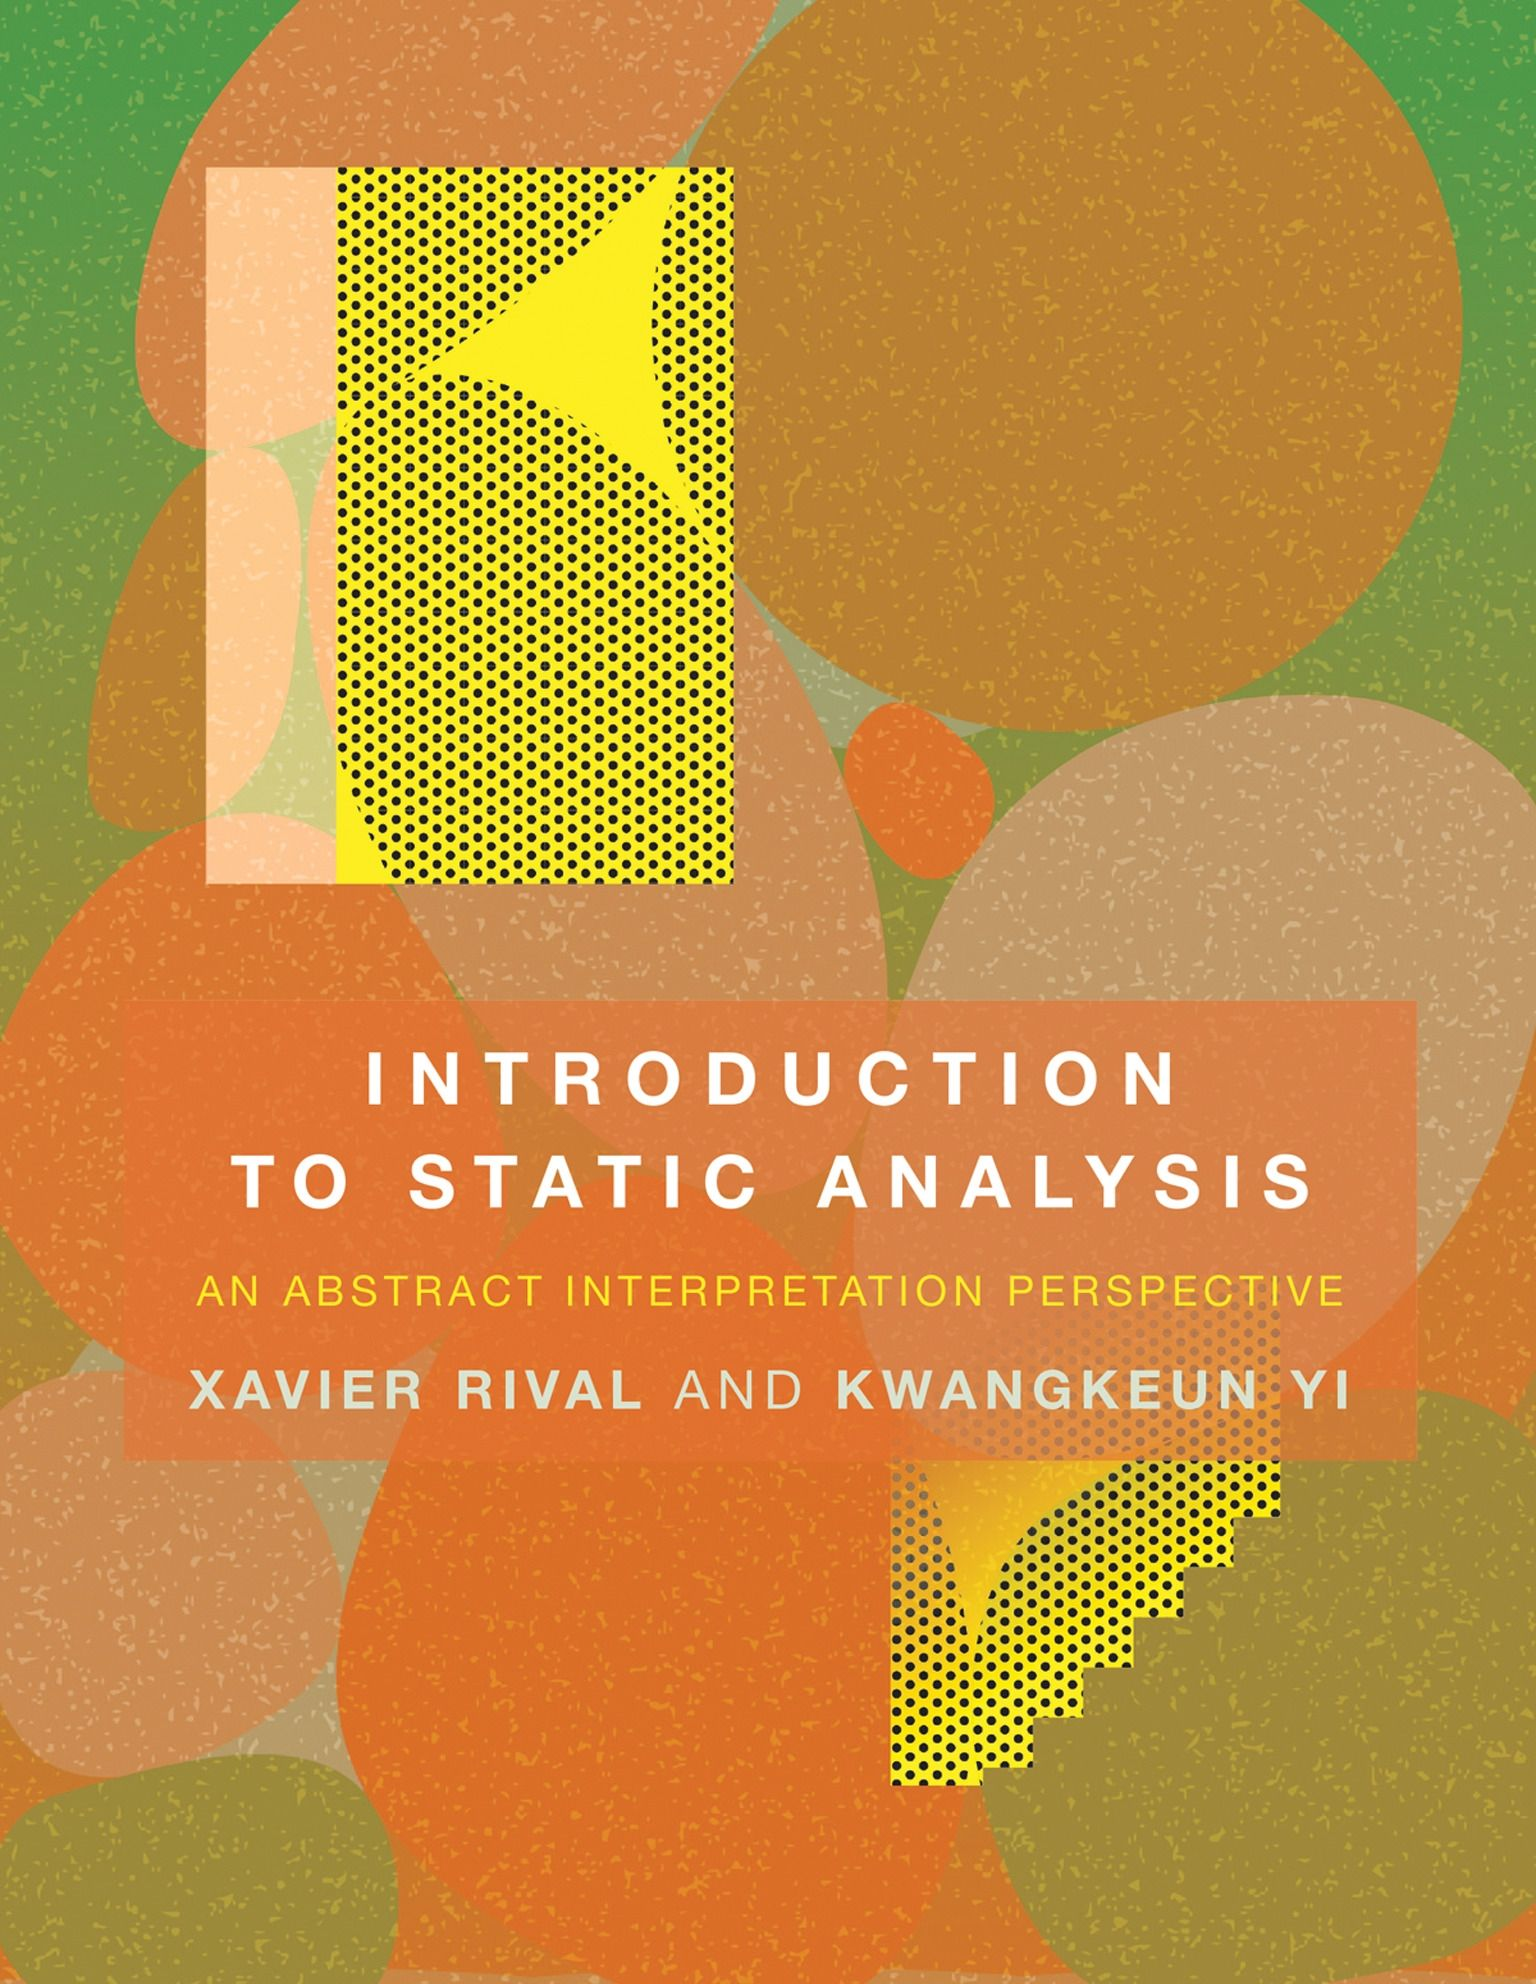
\includegraphics[width=4cm]{itsa-cover.jpg}}] (0,0) rectangle ++(3.8,5);
      \node[above] at(current bounding box.north) {\clap{\small\strut Using Analyses~\cite{rival2020introduction}}};
   }
\end{tikzpicture}}\hfill\raisebox{\dimexpr-\height+1cm}{\begin{tikzpicture}
   \onslide<3->{%
      \draw[darkgray,thick,rounded corners=2pt,path image={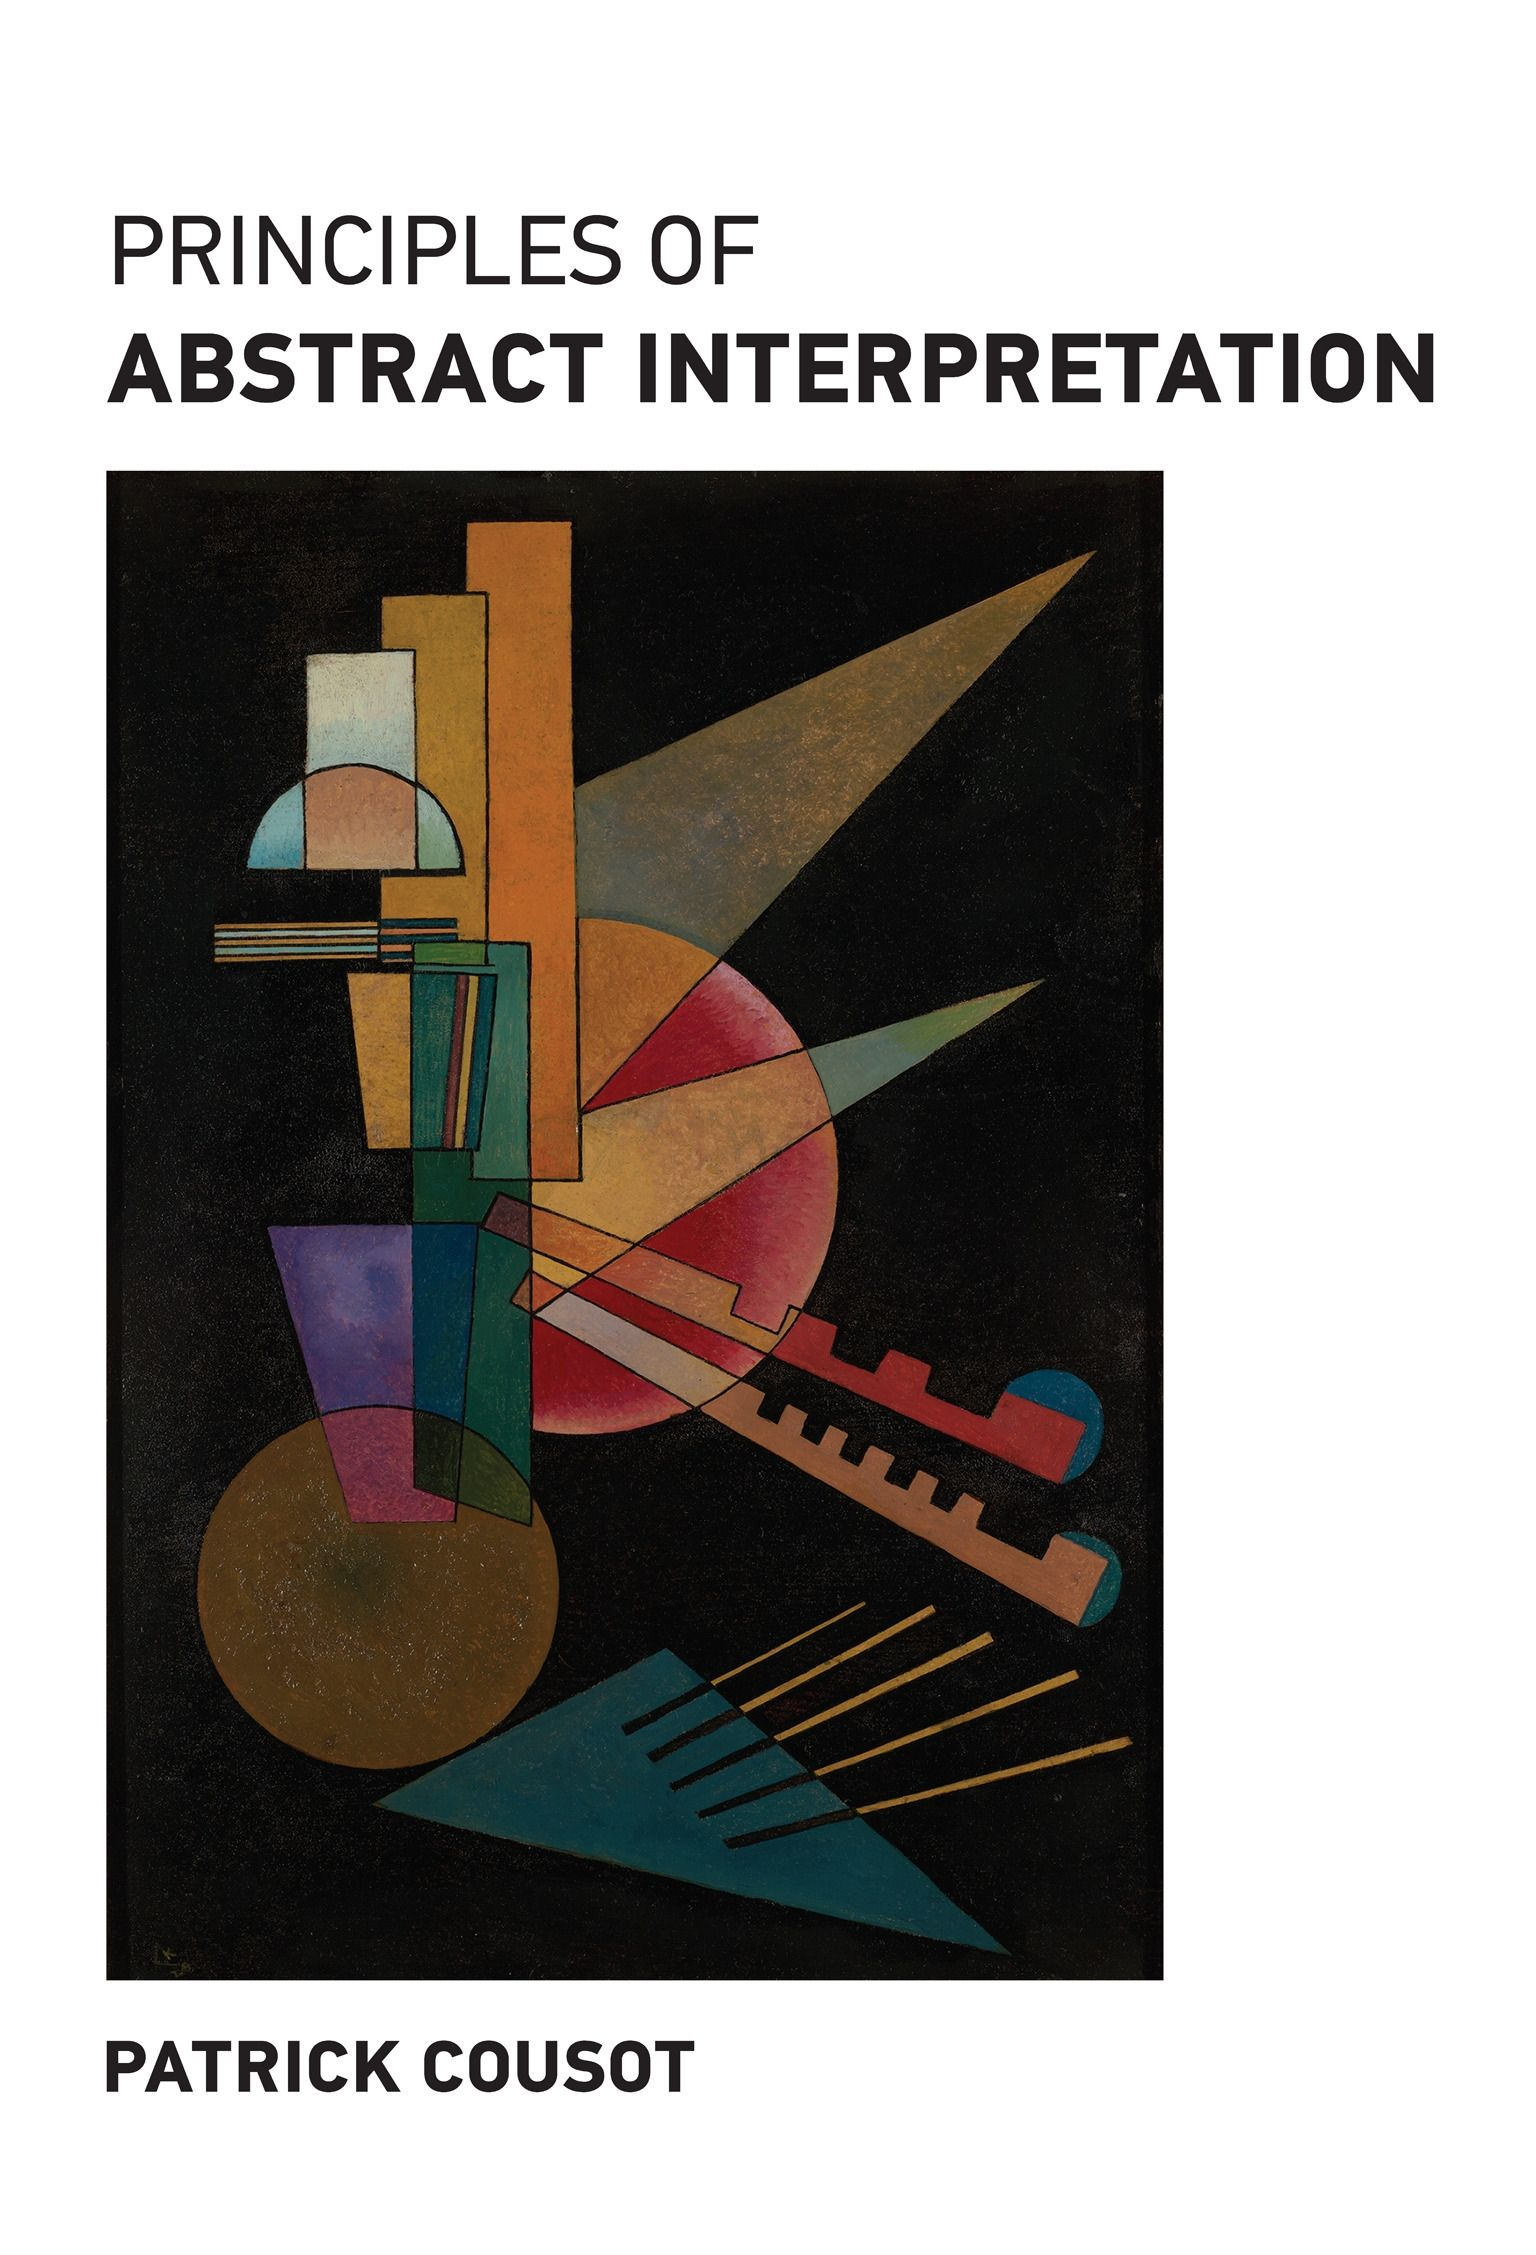
\includegraphics[width=4cm]{poa-cover.jpg}}] (0,0) rectangle ++(3.9,5.5);
      \node[above] at(current bounding box.north) {\clap{\small\strut Formal Foundations~\cite{cousout2021principles}}};
   }
\end{tikzpicture}}\hfill\raisebox{\dimexpr-\height+1cm}{\begin{tikzpicture}
   \onslide<4->{%
      \draw[darkgray,thick,rounded corners=2pt,path image={
\includegraphics[width=4cm]{dfa-cover.jpg}}] (0,0) rectangle ++(3.9,6);
      \node[above] at(current bounding box.north) {\clap{\small\strut Dataflow Perspective~\cite{10.5555/1592955}}};
   }
\end{tikzpicture}}\hfill\strut
\begin{tikzpicture}[overlay,remember picture]
   \node[above right=0.5mm,yshift=3mm,gray,font=\tiny] at (current page.south west) {And for an overview: \citetitle{DBLP:journals/ftpl/Mine17}~\cite{DBLP:journals/ftpl/Mine17}};
\end{tikzpicture}
\end{frame}

\section{The How}

\begin{frame}[fragile]{Abstract Interpretation}
\begin{uncoverenv}<2->
\AnimateCode{onslide={o2:{3,...,7},-,-,-},first slide=2}
\begin{minted}[escapeinside=||,lineskip=1pt]{java}
public static void main(String[] args) {
    int a = 1; |\tikzmarknode{bmark@a1}{\strut}|
    double r = Math.random() * 10; |\tikzmarknode{bmark@r1}{\strut}|
    if (r > 5) { |\tikzmarknode{bmark@r2}{\strut}|
       a = 2; |\tikzmarknode{bmark@a2}{\strut}|
    }
    System.out.println(a); |\tikzmarknode{bmark@a3}{\strut}|
}
\end{minted}
\endAnimateCode
\begin{tikzpicture}[overlay,remember picture]
   \coordinate[yshift=2pt] (bmark@a1) at (pic cs:bmark@a1);
   \node[right=4cm] (bmark@a1) at (bmark@a1) {\AbstractInfo{a \in \Set{1}}};
   \coordinate[yshift=2pt] (bmark@r1) at (pic cs:bmark@r1);
   \node[right] at (bmark@r1-|bmark@a1.west) {\AbstractInfo{r \in \IntCO{0}{10}}};
   \coordinate[yshift=2pt] (bmark@a2) at (pic cs:bmark@a2);
   \node[right] at (bmark@a2-|bmark@a1.west) {\AbstractInfo{a \in \Set{2}}};
   \coordinate[yshift=2pt] (bmark@a3) at (pic cs:bmark@a3);
   \node[right] (bmark@set) at (bmark@a3-|bmark@a1.west) {\AbstractInfo{a \in \Set{1, 2}}};
   \node[right] at (bmark@set.east) {\(\to\)~\;Valid? Ok? Safe?};
   \onslide<3->{%
      \fill[white,opacity=0.9] ([yshift=2cm]current page.west) rectangle ([yshift=-2cm]current page.east);
      \node[text width=.8\paperwidth,align=left] at(current page.center) {\begin{itemize}
         \itemsep10pt
         \item<4-> We want to proof interesting properties of programs
         \begin{itemize}
            \itemsep5pt
            \item<5-> \textit{Dataflow Properties}\\Liveness, Fainting, Reaching Definitions,~\ldots
            \item<6-> \textit{Safety Properties}\\No Null Dereference, No Division by Zero,~\ldots % finite prefix if we find violation
            \item<7-> \textit{Numerical Properties}\\Signs, Intervals, Octagons, Polyhedra,~\ldots
            \item<8-> \ldots
         \end{itemize}
      \end{itemize}};
   }%
   \node[above right,gray,yshift=3.5mm,font=\tiny,text width=.9\paperwidth] at (current page.south west) {\citetitle{cousout2021principles}~\cite[p.~722]{cousout2021principles},\citetitle{DBLP:journals/annals/GiacobazziR22}~\cite[pp.~37]{DBLP:journals/annals/GiacobazziR22}};
\end{tikzpicture}
\end{uncoverenv}
\end{frame}


\subsection{Terminology}

\newsavebox\GraphHeaven
\begin{frame}[c]{Abstract \textcolor{gray}{Interpretation}}
\frametitle<1>{Abstract \textcolor{gray}{Interpretation}}%
\frametitle<2-|handout:1>{Concrete \textcolor{gray}{Interpretation}}%
\frametitle<11-|handout:1>{Abstract \textcolor{gray}{Interpretation}}%
% häufige Visualisierung
\begin{lrbox}{\GraphHeaven}
\pgfmathsetseed{42}%
\begin{tikzpicture}[line cap=round]
   \pgfonlayer{foreground}
   \draw[Kite-Kite,very thick] (0,3.5) node[below right,yshift=1mm] {{\onslide<3->{\(x(t)\)}}} |- (8,0) node[above left] {{\onslide<2->{\(t\)}}}; % time vs. x at tat time
   \endpgfonlayer
   \colorlet{@}{red}
   \onslide<4->{\only<5->{\colorlet{@}{gray}}\draw[very thick,@] (0,1) plot [smooth] coordinates {(0,1) (1,2) (2,1) (3,2) (4,1) (5,2) (6,1) (7,2) (8,1)}; % x(t)
   }
   \colorlet{@}{red}
   \onslide<5->{\only<6->{\colorlet{@}{gray}}\draw[very thick,@] (0,0) plot [smooth] coordinates {(0,0) (1,1) (2,2) (3,2) (4,2.5) (5,2.5) (6,.5) (7,.6) (8,.6)}; % x(t)
   }
   \colorlet{@}{red}
   \onslide<6->{\only<7->{\colorlet{@}{gray}}\draw[very thick,@] (0,1.5) plot [smooth] coordinates {(0,1.5) (1,2) (2,2.5) (3,2) (4,2) (5,2.5) (6,2.5) (7,2) (8,2.5)}; % x(t)
   }
   \onslide<8->{
      \foreach \i in {0,...,5} {
         \pgfmathsetmacro{\randA}{rnd*0.33}
         \pgfmathsetmacro{\randB}{rand*0.5}
         \pgfmathsetmacro{\randC}{rand*0.4}
         \draw[gray] (0,1.5+\randA) plot [smooth] coordinates {(0,1.5+\randA) (1,2-\randB) (2,2.5-\randA) (3,2-\randB) (4,2+\randA) (5,2.5) (6,2.5+\randA) (7,2-\randA) (8,2.5+\randB)} node[inner sep=0pt] (a-\i) {};
         \draw[gray] (0,0+\randA) plot [smooth] coordinates {(0,0+\randA) (1,1-\randB) (2,2-\randB) (3,2+\randC) (4,2.5-\randA) (5,2.5-\randB) (6,.5+\randC) (7,.6+\randB) (8,.6+\randC)} node[inner sep=0pt] (b-\i) {};
         \draw[gray] (0,1+\randB) plot [smooth] coordinates {(0,1-\randC) (1,2-\randB) (2,1+\randB) (3,2-\randA) (4,1+\randA) (5,2-\randB) (6,1) (7,2-\randC) (8,1+\randA)} node[inner sep=0pt] (c-\i) {};
      }
   }
   % fit to all nodes to get the bounding box
   \node[fit=(a-0) (a-1) (a-2) (a-3) (a-4) (a-5) (b-0) (b-1) (b-2) (b-3) (b-4) (b-5) (c-0) (c-1) (c-2) (c-3) (c-4) (c-5),inner sep=0pt] (big-ghost) {~};
   \onslide<9->{
      \draw[decorate,thick,decoration={brace,amplitude=5pt,raise=2pt},gray] (big-ghost.north east) -- (big-ghost.south east) node[midway,right=7pt,gray,align=left] (@doc) {Collecting Semantics\textsuperscript{\cite[91]{cousout2021principles}}};
   }
   \onslide<10->{
      \node[below right,xshift=-2mm,yshift=5mm,font=\footnotesize,text width=6cm,opacity=.5] at (@doc.south west) {\begin{itemize}
         \itemsep-1pt
         \item Maybe impossible to compute statically
         \item \ldots~or very expensive (\faCaretRight~\textit{dynamic})
         \item[\faCaretRight] Abstract Interpretation to the rescue
      \end{itemize}};
   }
   \pgfonlayer{background}
   \pgfinterruptboundingbox
   \only<11|handout:0>{
   \fill[red,opacity=.175,even odd rule] plot [smooth] coordinates {(0,0) (1,0.4) (2,0.5) (3,1) (4,.8) (5,1) (6,.1) (7,0.2) (8.03,.2) (8.03,3) (7,2.8) (6,3) (5,2.95) (4,2.85) (3,2.75) (2,2.65) (1,2.5) (0,2) } -- cycle; 
   }
   \only<12->{
   \fill[red,opacity=.175,even odd rule] plot [smooth] coordinates {(0,0) (1,0.4) (2,0.5) (3,1) (4,.8) (5,1) (6,.1) (7,0.2) (8.03,.2) (8.03,3) (7,2.8) (6,3) (5,2.95) (4,2.85) (3,2.75) (2,2.65) (1,2.5) (0,2) } -- cycle (6,1.85) circle[radius=4mm]; 
   }
   \onslide<11->{%
      \draw[Circle-,red,rounded corners=4pt] (7.75,2.9) -- ++(.35,.5) -- ++(.5,0) node[right,align=left] {(Trace) Abstraction\textsuperscript{\cite[92]{cousout2021principles}}\\[-2pt]\footnotesize\color{gray}just one of many};
   }
   \endpgfinterruptboundingbox
   \onslide<13->{
      \node (@b1) at (6,1.85) {\small\faBug};
      \node (@b2) at (3,.35) {\small\faBug};
      \node (@b3) at (7,2.5) {\small\faBug};
   }
   \onslide<14->{
      \node[above left=-1mm,green] at(@b2.south east) {\scriptsize\faCheck};
   }
   \onslide<15->{
      \node[above left=-1mm,green] at(@b1.south east) {\scriptsize\faCheck};
   }
   \onslide<16->{
      \node[above left=-1mm,yshift=1pt,orange] at(@b3.south east) {\scriptsize\faQuestion};
   }
   \endpgfonlayer
   \path[use as bounding box] (0,0) rectangle (8,3.5);
\end{tikzpicture}
\end{lrbox}
\begin{tikzpicture}[overlay,remember picture]
   \node[xshift=2.5mm] at(current page.center) {\usebox\GraphHeaven};
   \node[above right,gray,yshift=3.5mm,font=\tiny,text width=.9\paperwidth] at (current page.south west) {See \citetitle{cousout2012casual}~\cite{cousout2012casual}};
\end{tikzpicture}
\end{frame}
\newsavebox\PowersetZHasse
\newsavebox\TestBox
% TOOD: measure and only box if larger?
\begin{lrbox}{\PowersetZHasse}
\def\S#1{\savebox\TestBox{\footnotesize\absexpr{\Set{#1}}}\ifdim\ht\TestBox>5mm\makebox[5mm][c]{\usebox\TestBox}\else\usebox\TestBox\fi}\color{gray}%
\begin{tikzpicture}
   \matrix (A) [matrix of nodes, row sep=1mm, column sep=-2mm]
   {
       & & & \kern-4mm\S{-4, 0, 1, 9}\kern-4mm & & & \\
       & & \S{-4,0,1} & \ldots & \S{0,1,9} & & \\
      & \S{-4,0} & \ldots & \S{0,1} & \ldots & \S{1,9} & \\
      \S{-4} & \ldots & \S{0} & \ldots & \S{1} & \ldots & \S{9} \\
      & & & \absexpr{\emptyset} & & & \\
   };
   \scope[line cap=round]
   \draw (A-1-4) -- (A-2-3) -- (A-3-2) -- (A-4-1) (A-4-1.south) -- (A-5-4);
   \draw (A-1-4) -- (A-2-5) -- (A-3-6) -- (A-4-7) (A-4-7.south) -- (A-5-4);
   \draw (A-3-2) -- (A-4-3) -- (A-3-4) (A-3-4) -- (A-4-5) -- (A-3-6);
   \draw (A-2-3) -- (A-3-4) -- (A-2-5);
   \draw (A-4-3) -- (A-5-4) -- (A-4-5);
   \draw[densely dotted] (A-5-4) -- ++(-1,0.05)  (A-5-4) -- ++(1,0.05);
   \foreach[count=\y] \i in {4,3,2,1} {
      \draw[densely dotted] (A-\y-\i.north west) -- ++(-.4,0.14);
      \node[left=3.5mm] at(A-\y-\i.west) {\footnotesize\ldots};
      \pgfmathsetmacro\other{int(8-\i)}
      \draw[densely dotted] (A-\y-\other.north east) -- ++(.4,0.14);
      \node[right=3.5mm] at(A-\y-\other.east) {\footnotesize\ldots};
   }
   \node[above=3.5mm] (pz) at(A-1-4.north) {\absexpr{\P(\Z)}};
   \draw[densely dotted] (pz) -- ++(-1.25,-0.1) (pz) -- ++(1.25,-0.1);
   \draw[-Kite] ([yshift=1cm,xshift=-3mm]current bounding box.south west) -- ([yshift=-5mm]current bounding box.north west) node[midway,left,font=\scriptsize] {\rotatebox{90}{\absexpr{\partof \asdef\eq \subseteq}}};
   \endscope
\end{tikzpicture}
\end{lrbox}
\begin{frame}{Terminology}
   \begin{itemize}
      \item \textsb{Property}\onslide<2->{ --- Set of states/traces that satisfy that property}\\
            \onslide<3->{\textcolor{gray}{Even integers: \absexpr{\text{P} = \Set{ z \in \Z \Given \exists k \in \Z : z = 2k} = \Set{0, 2, 4, 6, \ldots} \subseteq \P(\tikzmarknode{universe}{\Z})}}}
            \medskip

            \onslide<5->{\centerline{\absexpr{\tikzmarknode{ff}{\emptyset} \subseteq \tikzmarknode{p1}{\text{P}_1} \subseteq \tikzmarknode{p2}{\text{P}_2} \subseteq \tikzmarknode{tt}{\Universe}}}}
            \vspace*{4.9em}

      \item<10-> \textsb{Partial Order} \onslide<11->{--- A \tikzmarknode{reflexive}{reflexive}, \tikzmarknode{transitive}{transitive}, \tikzmarknode{antisymmetric}{antisymmetric} relation on a set}\\
            \textcolor{gray}{\onslide<15->{\absexpr{(\Z, \leq)}}\onslide<16->{,\quad\absexpr{(\P(\Z), \subseteq)},\quad\ldots}}
            % domains special kinds of partial orders
   \end{itemize}
   
   \begin{tikzpicture}[overlay,remember picture,line cap=round]
      \onslide<4->{
         \draw[Kite-,gray] ([yshift=-2pt]universe.south) to[out=310,in=180] ++(.4,-.25) node[right] {\small universe (\absexpr{\Universe})};
      }
      \onslide<6->{\draw[Kite-,gray] ([yshift=-2pt]ff.south) to[out=230,in=0] ++(-.4,-.25) node[left] {\small strongest};}
      \onslide<7->{\draw[Kite-,gray] ([yshift=-2pt,xshift=-2pt]p1.south) to[out=260,in=0] ++(-.4,-.55) node[left] {\small stronger};}
      \onslide<8->{\draw[Kite-,gray] ([yshift=-2pt,xshift=-2pt]p2.south) to[out=280,in=180] ++(.4,-.55) node[right] {\small weaker};}
      \onslide<9->{\draw[Kite-,gray] ([yshift=-2pt]tt.south) to[out=310,in=180] ++(.4,-.25) node[right] {\small weakest};}
      
      \onslide<12->{\draw[Kite-,gray] ([yshift=2pt]reflexive.north) to[out=130,in=0] ++(-.4,.215) node[left] {\small \absexpr{\forall x \in X : x \partof x}};}
      \onslide<13->{\draw[Kite-,gray] ([yshift=2pt]transitive.north) -- ++(0,.3) node[above=-1pt] {\small \absexpr{\forall x, y, z \in X : x \partof y \land y \partof z \implies x \partof z}};}
      \onslide<14->{\draw[Kite-,gray] ([yshift=2pt]antisymmetric.north) to[out=50,in=180] ++(.4,.215) node[right] {\kern-1pt\small\absexpr{\forall x, y \in X : x \partof y \land y \partof x \implies x = y}};}
      
      \node[above right,gray,yshift=3.5mm,font=\tiny,text width=.9\paperwidth] at (current page.south west) {\citetitle{cousout2021principles}~\cite[15]{cousout2021principles},\citetitle{DBLP:journals/ftpl/Mine17}~\cite[18]{DBLP:journals/ftpl/Mine17}};
      \onslide<17->{%
      \node[above left,yshift=3.5mm] at(current page.south east) {\scalebox{.65}{\usebox\PowersetZHasse}};
      }
   \end{tikzpicture}
\end{frame}

\begin{frame}[fragile]{Chains and Lattices}
\begin{onlyenv}<1|handout:0>
\begin{tikzpicture}
   \matrix (A) [matrix of nodes, row sep=2.5mm, column sep=-2mm]
   {
       & &  & \kern-4mm\S{-4, 0, 1, 9}\kern-4mm & & & \\
       & & \S{-4,0,1} & \ldots & \S{0,1,9} & & \\
      & \S{-4,0} & \ldots & \S{0,1} & \ldots & \S{1,9} & \\
      \S{-4} & \ldots & \S{0} & \ldots & \S{1} & \ldots & \S{9} \\
      & & & \absexpr{\emptyset} & & & \\
   };
   \scope[line cap=round]
   \draw (A-1-4) -- (A-2-3) -- (A-3-2) -- (A-4-1) (A-4-1.south) -- (A-5-4);
   \draw (A-1-4) -- (A-2-5) -- (A-3-6) -- (A-4-7) (A-4-7.south) -- (A-5-4);
   \draw (A-3-2) -- (A-4-3) -- (A-3-4) (A-3-4) -- (A-4-5) -- (A-3-6);
   \draw (A-2-3) -- (A-3-4) -- (A-2-5);
   \draw (A-4-3) -- (A-5-4) -- (A-4-5);
   \draw[densely dotted] (A-5-4) -- ++(-1,0.05)  (A-5-4) -- ++(1,0.05);
   \foreach[count=\y] \i in {4,3,2,1} {
      \draw[densely dotted] (A-\y-\i.north west) -- ++(-.4,0.14);
      \node[left=3.5mm] at(A-\y-\i.west) {\footnotesize\ldots};
      \pgfmathsetmacro\other{int(8-\i)}
      \draw[densely dotted] (A-\y-\other.north east) -- ++(.4,0.14);
      \node[right=3.5mm] at(A-\y-\other.east) {\footnotesize\ldots};
   }
   \node[above=3.5mm] (pz) at(A-1-4.north) {\absexpr{\P(\Z)}};
   \draw[densely dotted] (pz) -- ++(-1.25,-0.1) (pz) -- ++(1.25,-0.1);
   \draw[-Kite] ([yshift=1cm,xshift=-3mm]current bounding box.south west) -- ([yshift=-5mm]current bounding box.north west) node[midway,left,font=\scriptsize] {\rotatebox{90}{\absexpr{\partof \asdef\eq \subseteq}}};
   \endscope
\end{tikzpicture}
\end{onlyenv}
\begin{onlyenv}<2-|handout:1>
\begin{tikzpicture}
   \matrix (A) [matrix of nodes, row sep=2.5mm, column sep=-2mm]
   {
       & &  & \I{-1}{\infty} & & & \\
       & & \I{-1}{1} & \ldots & \I{0}{9} & & \\
      & \I{-1}{0} & \ldots & \I{0}{1} & \ldots & \I{1}{9} & \\
      \I{-1}{-1} & \ldots & \I00 & \ldots & \I11 & \ldots & \I99 \\
      & & & \absexpr{\bot} & & & \\
   };
   \scope[line cap=round]
   \draw (A-2-3) -- (A-3-2) -- (A-4-1) -- (A-5-4);
   \draw (A-3-6) -- (A-4-7) -- (A-5-4);
   \draw (A-3-2) -- (A-4-3) -- (A-3-4) (A-3-4) -- (A-4-5) -- (A-3-6);
   \draw (A-2-3) -- (A-3-4);
   \draw (A-4-3) -- (A-5-4) -- (A-4-5);
   \draw[densely dotted] (A-2-5) -- (A-1-4) -- (A-2-3) (A-3-4) -- (A-2-5) -- (A-3-6);
   \draw[densely dotted] (A-5-4) -- ++(-1,0.05)  (A-5-4) -- ++(1,0.05);
   \foreach[count=\y] \i in {4,3,2,1} {
      \draw[densely dotted] (A-\y-\i.north west) -- ++(-.4,0.14);
      \node[left=3.5mm] at(A-\y-\i.west) {\footnotesize\ldots};
      \pgfmathsetmacro\other{int(8-\i)}
      \draw[densely dotted] (A-\y-\other.north east) -- ++(.4,0.14);
      \node[right=3.5mm] at(A-\y-\other.east) {\footnotesize\ldots};
   }
   \node[above=3.5mm] (pz) at(A-1-4.north) {\absexpr{\top}};
   \draw[densely dotted] (pz) -- ++(-1.25,-0.1) (pz) -- ++(1.25,-0.1);
   \draw[-Kite] ([yshift=1cm,xshift=-3mm]current bounding box.south west) -- ([yshift=-5mm]current bounding box.north west) node[midway,left,font=\scriptsize] {\rotatebox{90}{\absexpr{\partof \asdef\eq \dot\subseteq}}};
   \endscope
   \pgfonlayer{background}
   \scope[opacity=.175,transparency group]
   \onslide<6->{%
      \draw[red,line width=3mm,rounded corners=2mm,line cap=round] (pz.center) -- ++(1.25,-.42) coordinate (@edge) -- (A-1-4.center) -- (A-2-3.center) -- (A-3-2.center) -- (A-4-1.center) -- (A-5-4.center);
      \foreach \i in {pz,A-1-4,A-2-3,A-3-2,A-4-1,A-5-4} {
         \fill[red,rounded corners=5pt,line cap=round] (\i.south west) rectangle (\i.north east);
      }
   }
   \endscope
   \onslide<4->{
      \draw[Kite-,red,rounded corners=4pt] ([xshift=1.5mm,yshift=-1mm]A-3-4.north) -- ++(.25,.325) -- ++(3,0) node[below right,yshift=.7\baselineskip,align=left] {Least upper bound\\[-2pt]\footnotesize\color{gray}of \IntCC00 and \IntCC11\\[-3pt]\footnotesize\color{gray}lub, join, \absexpr{\lub}};
   }
   \onslide<5->{
      \draw[Kite-,red,rounded corners=4pt] ([xshift=1mm,yshift=1mm]A-4-3.south) -- ++(-.4,-.85) -- ++(-.25,0) node[below left,yshift=.7\baselineskip,align=right] {Greatest lower bound\\[-2pt]\footnotesize\color{gray}of \IntCC{-1}{0} and \IntCC01\\[-3pt]\footnotesize\color{gray}glb, meet, \absexpr{\glb}};
   }
   \onslide<6->{
      \draw[Circle-,red,rounded corners=4pt] ([xshift=-1mm]@edge) -- ++(.35,.5) -- ++(.5,0) node[below right,yshift=.7\baselineskip,align=left] {Chain\\[-2pt]\footnotesize\color{gray}a totally ordered subset\\[-4pt]{\footnotesize\color{gray}\onslide<7->{e.g., \absexpr{\IntCC{0}{0} \partof \IntCC{0}{9} \partof \IntCC{-10}{200}}}}};
   }
   \endpgfonlayer
   \pgfinterruptboundingbox
   \onslide<3->{%
      \draw[Kite-,gray] (A-5-4.south) to[out=-60,in=180] ++(.5,-.25) node[right,font=\scriptsize] {bottom, empty interval};
      \draw[Kite-,gray] (pz.north) to[out=120,in=0] ++(-.5,.25) node[left,font=\scriptsize] {top, \absexpr{\IntCC{-\infty}{\infty}}};
   }
   \endpgfinterruptboundingbox
\end{tikzpicture}
\begin{tikzpicture}[overlay,remember picture]
\onslide<8->{%
   \node[above left,yshift=4.345mm,text width=5.5cm] at(current page.south east) {\textsb{Complete Lattice} \absexpr{(X, \partof, \lub, \glb, \bot, \top)}\vspace{-3.5mm}\footnotesize
   {\begin{itemize} 
      \itemsep-1pt
      \item<9-> \absexpr{(X, \partof)} is a partial order
      \item<10-> \absexpr{\forall A \subseteq X : \lub A} and \absexpr{\glb A} exist
      \item<11-> \absexpr{\bot}/\absexpr{\top} as smallest/largest element
   \end{itemize}}
   };
}
\end{tikzpicture}
\end{onlyenv}
% birkhoff1940lattice
\begin{tikzpicture}[overlay,remember picture]
   \node[above right,gray,yshift=3.5mm,font=\tiny,text width=.9\paperwidth] at (current page.south west) {\citetitle{birkhoff1967lattice}~\cite{birkhoff1967lattice}, see also sublattices~\cite[25]{DBLP:journals/ftpl/Mine17}};
\end{tikzpicture}
\end{frame}

\subsection{Abstract Domains}
\begin{frame}{\insertsubsection~\qquad\textcolor{gray}{Numerical}}
\vspace*{3.5em}
\tikzset{@/.style={red}}\only<5->{\tikzset{@/.style={gray}}}%
\begin{tikzpicture}[line cap=round]
   \draw[-Kite] (0,-1) -- (0,1) node[below left] {\scriptsize y};
   \draw[-Kite] (-1,0) -- (1,0) node[below left] {\scriptsize x};
\scope[@]
\onslide<2->{%
   \fill (.1,.1) coordinate (@) circle[radius=1.5pt];
   \foreach \x/\y in {.2/.3,-.1/.2,-.3/-.2,.2/-.5,.5/.4,-.8/.7,-.9/-.4,.4/.4,.35/-.4,-.4/.3} {
      \fill (\x,\y) circle[radius=1.5pt];
      \draw[-{Kite[scale=.4]}] (@) -- (\x,\y) coordinate (@);
   }
}
\onslide<3->{%
   \fill (-.4,-.55) circle[radius=1.5pt];
   \fill (.5,-.8) circle[radius=1.5pt];
   \draw[-{Kite[scale=.4]}] (-.4,-.55) -- (.5,-.8);
}
\endscope
\onslide<4->{%
   \node[below=1mm] at(current bounding box.south) {\scriptsize Collecting Semantics};
}
\end{tikzpicture}\hfill\onslide<5->{%
\tikzset{@/.style={red}}\only<8->{\tikzset{@/.style={gray}}}%
\begin{tikzpicture}[line cap=round]
   \draw[-Kite] (0,-1) -- (0,1) node[below left] {\scriptsize y};
   \draw[-Kite] (-1,0) -- (1,0) node[below left] {\scriptsize x};
\pgfonlayer{background}
\scope[@]
\onslide<6->{%
   \fill[@,opacity=.4] (-.4,-1) rectangle (.7,1);
   \draw[gray,thin] (-.4,-1) -- ++(0,2);
   \draw[gray,thin] (.7,-1) -- ++(0,2);
}
\endscope
\endpgfonlayer
\onslide<7->{%
   \node[below=1mm] at(current bounding box.south) {\clap{\scriptsize Intervals \absexpr{x \in \IntCC ab}}};
}
\end{tikzpicture}}\hfill\onslide<9->{%
\tikzset{@/.style={red}}\only<11->{\tikzset{@/.style={gray}}}%
\begin{tikzpicture}[line cap=round]
   \draw[-Kite] (0,-1) -- (0,1) node[below left] {\scriptsize y};
   \draw[-Kite] (-1,0) -- (1,0) node[below left] {\scriptsize x};
\scope[@]
\onslide<10->{%
   \foreach \x in {-1,-.7,...,1} {
      \foreach \y in {-.9,-.6,...,1} {
         \fill (\x,\y) circle[radius=1.5pt];
      }
   }
}
\endscope
\onslide<10->{%
   \node[below=1mm] at(current bounding box.south) {\clap{\scriptsize Simple Congruences}};
}
\end{tikzpicture}}\hfill\onslide<11->{%
\tikzset{@/.style={red}}\only<13->{\tikzset{@/.style={gray}}}%
\begin{tikzpicture}[line cap=round]
   \draw[-Kite] (0,-1) -- (0,1) node[below left] {\scriptsize y};
   \draw[-Kite] (-1,0) -- (1,0) node[below left] {\scriptsize x};
\scope[@]
\onslide<12->{%
   \fill[opacity=.4,@] (-.5,-.3) |- ++(.8,.6) -- ++(0,-.4) -- ++(-.2,-.2) -- cycle;
   \draw[gray,thin] (-.5,-.3) |- ++(.8,.6) -- ++(0,-.4) -- ++(-.2,-.2) -- cycle;
   \draw[thick,@] (.6,.2) -- ++(-.8,-.8);
}
\endscope
\onslide<12->{%
   \node[below=1mm] at(current bounding box.south) {\clap{\scriptsize Pentagons}};
}
\end{tikzpicture}}
\medskip
\begin{multicols}{4}
\begin{itemize}
   \item<14-> Octagons
   \item<15-> Ellipses
   \item<16-> Exponentials
   \item<17-> Signs
\end{itemize}
\end{multicols}
\begin{tikzpicture}[overlay,remember picture]
   \node[above right,gray,yshift=3.5mm,font=\tiny,text width=.9\paperwidth] at (current page.south west) {\citetitle{cousout2021principles}~\cite{cousout2021principles}, \citetitle{DBLP:conf/sac/LogozzoF08}~\cite[25]{DBLP:conf/sac/LogozzoF08}};
\end{tikzpicture}
% non relational: pointer, shapes, cost, ...
\end{frame}

\subsection{Sign Analysis}
\begin{frame}[fragile]{\insertsubsection\hfill\textcolor{gray}{Simple Sign Domain}}
\begin{itemize}
   \item<3-> We still have no program semantics, but we can try\ldots
\begin{minted}[escapeinside=||,lineskip=1pt]{java}
int a = 0; |\tikzmark{n@a1}|
int b = 12; |\tikzmark{n@b1}|
int c = a + b; |\tikzmark{n@c1}|
int d = c - b; |\tikzmark{n@d1}|
\end{minted}
\begin{tikzpicture}[overlay,remember picture]
   \onslide<4->{%
      \coordinate (n@a1) at (pic cs:n@a1);
      \node[right=2cm] (n@a1) at (n@a1) {\AbstractInfo{a = 0}};
   }%
   \onslide<5->{%
      \coordinate (n@b1) at (pic cs:n@b1);
      \node[right] at (n@b1-|n@a1.west) {\AbstractInfo{b \geq 0}};
   }%
   \onslide<6->{%
      \coordinate (n@c1) at (pic cs:n@c1);
      \node[right] at (n@c1-|n@a1.west) {\AbstractInfo{c \geq 0\quad (={} 0~{}+{}\geq 0)}};
   }%
   \onslide<7->{%
      \coordinate (n@d1) at (pic cs:n@d1);
      \node[right] (n@d1) at (n@d1-|n@a1.west) {\AbstractInfo{d = \top\kern-1.5pt\quad (\geq{} 0~{}-{}\geq 0)}};
   }
\end{tikzpicture}
   \item<8-> But how to handle control flow? Loops? Recursion?
\end{itemize}

\begin{tikzpicture}[overlay,remember picture]
   \onslide<2->{\node[above left=.5mm,yshift=3.5mm] at(current page.south east) {\usebox\SimpleSignLattice};}
\end{tikzpicture}
\end{frame}


\subsection{Fixpoints}
\begin{frame}{\insertsubsection}
   \begin{itemize}
      \itemsep10pt
      \item<2-> For operators \(f: X \to X\) a \textsb{fixpoint} is a \(x \in X\) such that \(f(x) = x\)
      \item<3-> If we iterate \(f\) starting from some \(x_0 \in X\):\medskip
      \begin{itemize}[--]
         \itemsep15pt
         \item<4-> \parbox{3.25cm}{\smash{\tikz[baseline=-.85mm,gray]{\coordinate (@) at (0,0);\fill (@) circle[radius=2pt] node[below] {\tiny\(x_0\)};\foreach \i in {0,...,3} {
            \draw[-Kite] (@) -- ++(.5,0) coordinate[xshift=1pt] (@);
            \fill (@) circle[radius=2pt] node[below] {\tiny\(f_\i\)};
         }; \draw[Kite-] ([xshift=-1pt]@) to[out=120,in=60,looseness=10] ([xshift=2pt]@);}}} \onslide<5->{reach a fixpoint, \(f^p = f(f^p)\)}%\hfill\textcolor{gray}{\footnotesize\absexpr{f : \N \to \N, f(x) = x}}
         \item<6-> \parbox{3.25cm}{\smash{\tikz[baseline=-.85mm,gray]{\coordinate (@) at (0,0);\fill (@) circle[radius=2pt] node[below] {\tiny\(x_0\)};\foreach \i in {0,...,3} {
            \draw[-Kite] (@) -- ++(.5,0) coordinate[xshift=1pt] (@) coordinate (@\i);
            \fill (@) circle[radius=2pt] node[below] {\tiny\(f_\i\)};
         }; \draw[-Kite] (@) to[out=70,in=60] (@1);}}} \onslide<7->{reach a cycle, \(f^{p + \ell} = f^p, \ell > 0\)}% \hfill\textcolor{gray}{\footnotesize\absexpr{f : \N \to \N, f(x) = x + 1}}
         \item<8-> \parbox{3.25cm}{\smash{\tikz[baseline=-.85mm,gray]{\coordinate (@) at (0,0);\fill (@) circle[radius=2pt] node[below] {\tiny\(x_0\)};\foreach \i in {0,...,3} {
            \draw[-Kite] (@) -- ++(.5,0) coordinate[xshift=1pt] (@) coordinate (@\i);
            \fill (@) circle[radius=2pt] node[below] {\tiny\(f_\i\)};
         }; \draw[densely dotted,semithick] (@) -- ++(0.42,0)}}} \onslide<9->{iterate forever, \(\forall p \neq q \in \mathbb{N} : f^{p} \neq f^q\)}\hfill\textcolor{gray}{\footnotesize\absexpr{f : \N \to \N, f(x) = x + 1}}
      \end{itemize}
      \item<10-> If our function is monotonic, we can always find a fixpoint\textsuperscript{\cite{tarski1955lattice}} \tikzmarknode{tarski}{\strut}
      \item<12-> Analyzing, e.g. loops, we \enquote{go up} the lattice until we reach a least fixpoint
   \end{itemize}
\begin{tikzpicture}[overlay,remember picture]
   \node[above right,gray,yshift=3.5mm,font=\tiny,text width=.9\paperwidth] at (current page.south west) {\citetitle{tarski1955lattice}~\cite{tarski1955lattice}, \citetitle{kleene1952introduction}~\cite{kleene1952introduction}, \citetitle{cousout2021principles}~\cite[165]{cousout2021principles}};
   \onslide<11->{%
      \draw[-Kite,line cap=round,gray] ([yshift=1.5pt]pic cs:tarski) to[out=0,in=180] ++(.5,.25) node[right,font=\tiny,align=left] {for complete, nonempty lattices\\Tarksi's Theorem};
   }
\end{tikzpicture}
\note[itemize]{
   \item Fixpunkte ganz ähnlich zu LaTeX - kompilierdurchläufe bis keine Änderungen mehr
}
\end{frame}

\subsection{Interval Analysis, I}

\begin{lrbox}{\SimpleSignLattice}
\scriptsize
\begin{tikzpicture}[line cap=round,x=6.5mm,y=6.5mm,gray]
   \node (top) at (0,0) {\absexpr{\top}};
   \node (pos) at (-1,-1) {\absexpr{\geq 0}};
   \node (neg) at (1,-1) {\absexpr{\leq 0}};
   \node (zero) at (0,-2) {\absexpr{0}};
   \node (bot) at (0,-3) {\absexpr{\bot}};
   \draw (top) -- (pos) -- (zero) -- (neg) -- (top) (zero) -- (bot);
\end{tikzpicture}
\end{lrbox}
\newsavebox\IntervalLattice

\def\mark{\color{red}\let\I\MarkedI}
\def\MarkedI#1#2{\footnotesize\absexpr{\mathbf{\IntCC{#1}{#2}}}}
\begin{frame}[fragile]{\insertsubsection}
\begin{lrbox}{\IntervalLattice}
\scriptsize
\begin{tikzpicture}[line cap=round,x=6.5mm,y=6.5mm,gray]
   \matrix (A) [matrix of nodes, row sep=2.5mm, column sep=-2mm]
   {
       & &  & \I{-1}{\infty} & & & \\
       & & \I{-1}{1} & \ldots & \only<12-|handout:3>{\mark}\I{0}{2} & & \\
      & \I{-1}{0} & \ldots & \only<9-11|handout:2>{\mark}\I{0}{1} & \ldots & \I{1}{2} & \\
      \I{-1}{-1} & \ldots & \only<4-8|handout:1>{\mark}\I00 & \ldots & \only<7-8|handout:1>{\mark}\I11 & \ldots & \I22 \\
      & & & \absexpr{\bot} & & & \\
   };
   \scope[line cap=round]
   \draw (A-2-3) -- (A-3-2) -- (A-4-1) -- (A-5-4);
   \draw (A-3-6) -- (A-4-7) -- (A-5-4);
   \draw (A-3-2) -- (A-4-3) -- (A-3-4) (A-3-4) -- (A-4-5) -- (A-3-6);
   \draw (A-2-3) -- (A-3-4) (A-3-4) -- (A-2-5) -- (A-3-6);
   \draw (A-4-3) -- (A-5-4) -- (A-4-5);
   \draw[densely dotted] (A-2-5) -- (A-1-4) -- (A-2-3);
   \draw[densely dotted] (A-5-4) -- ++(-1,0.05)  (A-5-4) -- ++(1,0.05);
   \foreach[count=\y] \i in {4,3,2,1} {
      \draw[densely dotted] (A-\y-\i.north west) -- ++(-.4,0.14);
      \node[left=3.5mm] at(A-\y-\i.west) {\footnotesize\ldots};
      \pgfmathsetmacro\other{int(8-\i)}
      \draw[densely dotted] (A-\y-\other.north east) -- ++(.4,0.14);
      \node[right=3.5mm] at(A-\y-\other.east) {\footnotesize\ldots};
   }
   \node[above=3.5mm] (pz) at(A-1-4.north) {\absexpr{\top}};
   \draw[densely dotted] (pz) -- ++(-1.25,-0.1) (pz) -- ++(1.25,-0.1);
   \endscope
\end{tikzpicture}
\end{lrbox}\vspace*{-2em}%
\begin{minted}[escapeinside=||,lineskip=1pt]{java}
int x = 0; |\tikzmark{int@i1}\medskip|
while(x < 2) {|\tikzmark{int@i2}\medskip|
   x = x + 1; |\tikzmark{int@i3}|
}|\tikzmark{int@i4}|
\end{minted}
\begin{tikzpicture}[overlay,remember picture]
   \onslide<3->{%
      \coordinate[yshift=2pt] (int@i1) at (pic cs:int@i1);
      \node[right=2cm] (int@i1) at (int@i1) {\AbstractInfo{x_0 \in \IntCC00 }};
   }%
   \onslide<5->{%
      \coordinate[yshift=2pt] (int@i2) at (pic cs:int@i2);
      \node[above right,yshift=-1.5pt] (int@i2a) at (int@i2-|int@i1.west) {\AbstractInfo{\only<8-9,12|handout:2,3>{\boldmath}\text{\textcolor{gray}{\scriptsize[pre]}~}x_1 \in \only<-8|handout:1>{\IntCC00}\only<9-11|handout:2>{\IntCC01\quad (\IntCC00 \cup \IntCC11)}\only<12-|handout:3>{\IntCC02\quad (\IntCC01 \cup \IntCC12)}}};
   }%
   \onslide<6->{%
      \node[below right,yshift=1.5pt] (int@i3a) at (int@i2-|int@i1.west) {\AbstractInfo{\only<10|handout:0>{\boldmath}\text{\textcolor{gray}{\scriptsize[in]}~}x_2 \in \only<-9|handout:1>{\IntCC00\quad (\IntCC00 \cap \IntOC{-\infty}1)}\only<10-|handout:2>{\IntCC01\quad (\IntCC01 \cap \IntOC{-\infty}1)}}};
   }%
   \onslide<7->{%
      \coordinate[yshift=2pt] (int@i3) at (pic cs:int@i3);
      \node[right] (int@i3) at (int@i3-|int@i1.west) {\AbstractInfo{\only<11|handout:0>{\boldmath}\text{}x_3 \in \only<-10|handout:1>{\IntCC11\quad (\IntCC00 \oplus \IntCC11)}\only<11-|handout:2>{\IntCC12\quad (\IntCC01 \oplus \IntCC11)}}};
   }
   \onslide<13-|handout:3>{%
      \coordinate[yshift=2pt] (int@i4) at (pic cs:int@i4);
      \node[right] (int@i4) at (int@i4-|int@i1.west) {\AbstractInfo{\text{\textcolor{gray}{\scriptsize[post]}~}x_4 \in \IntCC22 \quad (\IntCC02 \cap \IntCO2{\infty})}};
   }
   \onslide<14-|handout:3>{
      \node[right=4.5cm] (int@i1@sign) at (int@i1.east) {\AbstractInfo{x_0 = 0}};
      \node[right] at (int@i2a-|int@i1@sign.west) {\AbstractInfo{\text{\textcolor{gray}{\scriptsize[pre]}~}x_1 \geq 0}};
      \node[right] at (int@i3a.east-|int@i1@sign.west) {\AbstractInfo{\text{\textcolor{gray}{\scriptsize[in]}~}x_2 \geq 0}};
      \node[right] at (int@i3-|int@i1@sign.west) {\AbstractInfo{x_3 \geq 0}};
      \node[right] at (int@i4-|int@i1@sign.west) {\AbstractInfo{\text{\textcolor{gray}{\scriptsize[post]}~}x_4 \geq 0}};
      \node[above] at(int@i1@sign.north) {\footnotesize Signs};
      \node[above] at(int@i1.north) {\footnotesize Intervals};
   }
\end{tikzpicture}

\begin{tikzpicture}[overlay,remember picture]
   \onslide<2->{\node[above left=.5mm,yshift=3.5mm] at(current page.south east) {\scalebox{.85}{\usebox\IntervalLattice}};}
   \onslide<15->{
      \node[above right=.5mm,yshift=3.5mm] at (current page.south west) {\scalebox{.85}{\usebox\SimpleSignLattice}};
   }
\end{tikzpicture}
\end{frame}

\section{Semantics}

\def\Comment#1{\kern-2pt\textcolor{gray}{\footnotesize(\absexpr{#1})}}
\def\Kw#1{\textbf{\small#1}}
\def\stm{\mathcolor{red}{stm}}
\def\expr{\mathcolor{red}{expr}}
\def\cond{\mathcolor{red}{cond}}

\begin{frame}[fragile]{\insertsection}
\frametitle<2-|handout:1>{\textcolor{gray}{Semantics}\qquad Program Syntax (simplified)}
\begin{uncoverenv}<3-|handout:1>
\begin{minted}[lineskip=14pt,escapeinside=||]{java}
int |\tikzmarknode{sem-var-x}{\strut}|x |\tikzmarknode{sem-assign}{\strut}|= |\tikzmarknode{sem-num-const}{\strut}|0;|\tikzmarknode{sem-seq}{\strut}|
|\tikzmarknode{sem-loop}{\strut}|while(x |\tikzmarknode{sem-bin-cmp}{\strut}|< 2) {
   x = x |\tikzmarknode{sem-bin-exp}{\strut}|+ 1;
}
\end{minted}
\begin{tikzpicture}[overlay,remember picture,line cap=round,gray]
   \onslide<4->{%
      \draw[Kite-] ([xshift=2.85pt,yshift=6pt]pic cs:sem-var-x) to[out=60,in=180] ++(.5,.6) node[right,font=\scriptsize] {Variable~\absexpr{v \in \Variables}};
   }
   \onslide<5->{%
      \draw[Kite-] ([xshift=2.85pt,yshift=5pt]pic cs:sem-assign) to[out=50,in=180] ++(.5,.25) node[right,font=\scriptsize] {Assignment};
   }
   \onslide<6->{%
      \draw[Kite-] ([xshift=3pt,yshift=-.5pt]pic cs:sem-num-const) to[out=-50,in=180] ++(.5,-.3) node[right,font=\scriptsize] {Numeric Constant~\absexpr{c\in \NumericDomain}};
   }
   \onslide<7->{%
      \draw[Kite-] ([xshift=1pt]pic cs:sem-seq) -- ++(0.42,0) node[right,font=\scriptsize] {Sequence};
   }
   \onslide<8->{%
      \draw[Kite-] ([xshift=13pt,yshift=7.5pt]pic cs:sem-loop) to[out=70,in=180] ++(.25,.3) node[right,font=\scriptsize] {Loop};
   }
   \onslide<9->{%
      % sem-bin-cmp
      \draw[Kite-] ([xshift=3pt,yshift=-1pt]pic cs:sem-bin-cmp) to[out=-50,in=180] ++(.5,-.25) node[right,font=\scriptsize] {Comparison \absexpr{\AnyCompare \in \{\leq, <, ~\ldots\}}};
   }
   \onslide<10->{
      \draw[Kite-] ([xshift=3pt,yshift=-.5pt]pic cs:sem-bin-exp) to[out=-50,in=180] ++(.5,-.25) node[right,font=\scriptsize] {Binary Expression};
   }
\end{tikzpicture}
\end{uncoverenv}
% https://craftinginterpreters.com/representing-code.html#rules-for-grammars
\begin{tikzpicture}[overlay,remember picture]
   \node[above right,gray,yshift=3.5mm,font=\tiny,text width=.9\paperwidth] at (current page.south west) {Shortened form of \citetitle{DBLP:journals/ftpl/Mine17}~\cite[46]{DBLP:journals/ftpl/Mine17}, \href{https://web.archive.org/web/20241121192150/https://craftinginterpreters.com/representing-code.html#rules-for-grammars}{craftinginterpreters.com/representing-code.html}};
   \onslide<11->{
      \node[left=2mm] at(current page.east) {\small
\begin{bnf}
\(\stm\) ::=
   | \absexpr{V \leftarrow \expr} : \Comment{\text{assignment}, V \in \Variables}
   | \absexpr{\stm_1;~\stm_2} : \Comment{\text{sequence}}
   | \absexpr{\Kw{while}(\cond)~\{~\stm~\}} : \Comment{\text{loop}}
   ;;
\(\expr\) ::=
   | \(V\) : \Comment{\text{variable}, V \in \Variables}
   | \(c\) : \Comment{\text{constant}, c \in \NumericDomain}
   | \(\expr_1 \diamond \expr_2\) : \Comment{\text{bin. expr.}, \diamond \in \{+, -, ~\ldots\}}
   ;;
\(\cond\) ::= 
   | \(b\) : \Comment{\text{boolean}, b \in \BooleanDomain}
   | \(\expr_1 \bowtie \expr_2\) : \Comment{\text{comparison}, \bowtie \in \{\leq, <, ~\ldots\}}
   ;;
\end{bnf}
      };
   }
\end{tikzpicture}
\end{frame}

\begin{frame}[fragile,t]{Atomic Expression Semantics}
\begin{minted}[escapeinside=||]{java}
int |\tikzmarknode{bsem-var-x}{\strut}|x |\tikzmarknode{bsem-assign}{\strut}|= |\tikzmarknode{bsem-num-const}{\strut}|0;|\tikzmarknode{bsem-seq}{\strut}|
|\tikzmarknode{bsem-loop}{\strut}|while(x |\tikzmarknode{bsem-bin-cmp}{\strut}|< 2) {
   x = x |\tikzmarknode{bsem-bin-exp}{\strut}|+ 1;
}
\end{minted}
% https://craftinginterpreters.com/representing-code.html#rules-for-grammars
\begin{tikzpicture}[overlay,remember picture]
   \node[above right,gray,yshift=3.5mm,font=\tiny,text width=.9\paperwidth] at (current page.south west) {Shortened form of \citetitle{DBLP:journals/ftpl/Mine17}~\cite[46]{DBLP:journals/ftpl/Mine17}, \href{https://web.archive.org/web/20241121192150/https://craftinginterpreters.com/representing-code.html#rules-for-grammars}{craftinginterpreters.com/representing-code.html}};
      \node[left=2mm,yshift=6em] at(current page.east) {\small%
\begin{bnf}
\(\expr\) ::=
   | \(V\) : \Comment{\text{variable}, V \in \Variables}
   | \(c\) : \Comment{\text{constant}, c \in \NumericDomain}
   | \(\expr_1 \diamond \expr_2\) : \Comment{\text{bin. expr.}, \diamond \in \{+, -, ~\ldots\}}
   ;;
\end{bnf}
      };
\end{tikzpicture}\vspace*{-7mm}
\begin{itemize}
   \itemsep12pt
   \item<2-> We use an environment \absexpr{\Environments \asdef\eq \tikzmarknode{node@variables}{\Variables} \to \tikzmarknode{node@integers}{\NumericDomain}} to represent the current program state
   \item<6-> Now we can define \absexpr{\text{evalExpr}(\expr \tikzmarknode{formal-expr-eval}{\mathcolor{black}{,}}~env)} for an environment \absexpr{env \in \Environments}\vspace*{-1mm}
      {\small\begin{equation*}
         \begin{array}{lcl}
         \onslide<8->{\text{evalExpr}(V,~env)} &\onslide<8->{\absexpr{\asdef\eq}}& \onslide<8->{env(V)\tikzmarknode{value-by-env}{\strut}} \\
         \onslide<10->{\text{evalExpr}(c,~env)} &\onslide<10->{\absexpr{\asdef\eq}}& \onslide<10->{c} \\
         \onslide<11->{\text{evalExpr}(\expr_1 + \expr_2,~env)} &\onslide<11->{\absexpr{\asdef\eq}}& \onslide<11->{\text{evalExpr}(\expr_1,~env) + \text{evalExpr}(\expr_2,~env)} \\
         & \onslide<12->{\vdots} & 
      \end{array}
      \end{equation*}}
   \item<13-> Additionally we can define \absexpr{\text{evalCond}(\cond\tikzmarknode{formal-cond-eval}{\mathcolor{black}{,}}~envs)} and \absexpr{\text{evalStm}(\stm\tikzmarknode{formal-stm-eval}{\mathcolor{black}{,}}~envs)}
\end{itemize}  
\begin{tikzpicture}[overlay,remember picture,line cap=round]
\scope[gray]
\onslide<3->{%
\draw[Kite-] ([yshift=9pt]pic cs:node@variables) to[out=110,in=0] ++(-.5,.33) node[left,font=\scriptsize] {Variable};%
}
\onslide<4->{%
\draw[Kite-] ([yshift=9pt]pic cs:node@integers) to[out=70,in=180] ++(.5,.33) node[right,font=\scriptsize] {Integer Values};
}
\onslide<5->{
   \node[below left,xshift=-4mm,yshift=8.95mm,gray] at(current page.east) {\small%
      \begin{tabular}{l@{\hskip4pt}c}
         \absexpr{\Variables} & \absexpr{\NumericDomain} \\
         \hline
         \absexpr{x} & \absexpr{0} \\
         \absexpr{c} & \absexpr{5} \\
      \end{tabular} 
   };
}
\onslide<7->{%
   \draw[Kite-] ([yshift=8pt]pic cs:formal-expr-eval) to[out=110,in=0] ++(-.5,.25) node[left,font=\scriptsize] {Usually written as \absexpr{\EvaluateExpr{expr}\Environment}};
}
\onslide<9->{%
   \draw[Kite-] ([xshift=1pt,yshift=2pt]pic cs:value-by-env) to[out=10,in=190] ++(.6,.2) node[right,font=\scriptsize] {Value of \absexpr{V \in \Variables} in Environment~\(env\)};
}
\onslide<14->{%
   \draw[Kite-] ([yshift=8pt]pic cs:formal-cond-eval) to[out=120,in=0] ++(-.5,.25) node[left,font=\scriptsize] {\absexpr{\EvaluateCond{cond}\SetOfStates}};
}
\onslide<15->{%
   \draw[Kite-] ([yshift=8pt]pic cs:formal-stm-eval) to[out=120,in=0] ++(-.5,.25) node[left,font=\scriptsize] {\absexpr{\EvaluateStatement{stm}\SetOfStates}};
}
\endscope
\end{tikzpicture}
\end{frame}

\begin{frame}{Denotational Semantics\qquad \textcolor{gray}{while loops}}
   \begin{center}
      \hspace*{-14em}\onslide<2->{\tikzmarknode{while-loop-node}{\absexpr{\Kw{while}(\cond)~\{~\stm~\}}}}
   \end{center}
   % we reach fixpoint in the abstract due to tarki and kleene and the fact that we have this lfp on the chain. consideration afterwards does no longer have tro reflect infinite iteration as we intersect with the not condition fact
   \begin{tikzpicture}[overlay,remember picture,line cap=round]
      \onslide<3->{\draw[Kite-] (while-loop-node.north) -- ++(0,.35) node[above,font=\footnotesize] {Suppose we start the loop with states \absexpr{Start}};}
      \onslide<4->{%
         \draw[-Kite] (while-loop-node.south east) to[out=-30,in=30,looseness=6] node[pos=.5,right,align=left] {%
            \absexpr{F(X) \asdef\eq Start \cup evalStm(\stm,~evalCond(\cond,~X))}\\[-4pt]
            \color{gray}\scriptsize iterate to find the least fixpoint~\cite[52]{DBLP:journals/ftpl/Mine17}
         } (while-loop-node.north east);
      }
      \onslide<5->{%
         \draw[-Kite] ([yshift=-1pt]while-loop-node.south) -- ++(0,-.5)
            node[below,font=\footnotesize] {Keep only states~\absexpr{S} with \absexpr{evalCond(\lnot \cond,~S)}};
      }
      \onslide<6->{%
         \node[above=2cm] (@) at(current page.south) {There are alternatives (e.g., equation systems, \cite[part~7]{cousout2021principles})}; % denotational semantics follow the control flow
      }
      \onslide<7->{%
         \node[below=5mm,align=center,text width=.75\paperwidth] (@ad) at(@.south) {We achieve their abstract counterpart using the same principles but for abstract domains!};
      }
      \onslide<8->{
         \draw[Kite-,gray,line cap=round] ([yshift=2.75mm,xshift=-2.1cm]@ad.south east) to[out=20,in=180] ++(.4,.3) node[below right,font=\scriptsize,yshift=.7\baselineskip,align=left] {Usually written as\\\absexpr{\RawEvaluateStatement\isAbstract, \RawEvaluateCond\isAbstract, \RawEvaluateExpr\isAbstract,~\ldots}};
      }
   \end{tikzpicture}
\end{frame}

\subsection{Interval Analysis, II}
\begin{frame}[fragile]{\insertsubsection}
\begin{onlyenv}<1|handout:0>
\begin{minted}[escapeinside=||,lineskip=5pt]{java}
int x = 0;
while(x < 2) {
   x = x + 1;
}
\end{minted}
\end{onlyenv}
\begin{onlyenv}<2->
\begin{minted}[escapeinside=||,lineskip=5pt]{java}
int x = 0; |\tikzmark{long@i1}\medskip|
while(x < 999999) {|\tikzmark{long@i2}\medskip|
   x = x + 1;|\tikzmark{long@i3}|
}|\tikzmark{long@i4}|
\end{minted}
\begin{tikzpicture}[overlay,remember picture]
   \onslide<3->{%
      \coordinate[yshift=2pt] (long@i1) at (pic cs:long@i1);
      \node[right=2cm] (long@i1) at (long@i1) {\AbstractInfo{x_0 \in \IntCC00 }};
   }%
   \onslide<4->{%
      \coordinate[yshift=2pt] (long@i2) at (pic cs:long@i2);
      \node[above right,yshift=-1.5pt] (long@i2a) at (long@i2-|long@i1.west) {\AbstractInfo{\only<7-8,11-15>{\boldmath}\text{\textcolor{gray}{\scriptsize[pre]}~}x_1 \in \only<-7>{\IntCC00}\only<8-10>{\IntCC01\quad (\IntCC00 \cup \IntCC11)}\only<11->{\IntCC02\quad (\IntCC01 \cup \IntCC12)}}};
   }%
   \onslide<5->{%
      \node[below right,yshift=1.5pt] (long@i3a) at (long@i2-|long@i1.west) {\AbstractInfo{\only<9|handout:0>{\boldmath}\text{\textcolor{gray}{\scriptsize[in]}~}x_2 \in \only<-8>{\IntCC00\quad (\IntCC00 \cap \IntOC{-\infty}1)}\only<9->{\IntCC01\quad (\IntCC01 \cap \IntOC{-\infty}1)}}};
   }%
   \onslide<6->{%
      \coordinate[yshift=2pt] (long@i3) at (pic cs:long@i3);
      \node[right] (long@i3) at (long@i3-|long@i1.west) {\AbstractInfo{\only<10|handout:0>{\boldmath}\text{}x_3 \in \only<-9>{\IntCC11\quad (\IntCC00 \oplus \IntCC11)}\only<10->{\IntCC12\quad (\IntCC01 \oplus \IntCC11)}}};
   }
   \onslide<12->{%
      \node[right] at(long@i2a.east) {{\only<-14|handout:0>{\ldots}\only<15->{%
         \absexpr{\widen \implies x_1 \in \IntCO{0}{\infty}}
      }}};%
   };
   \onslide<16->{%
      \coordinate[yshift=2pt] (long@i4) at (pic cs:long@i4);
      \node[right] (long@i4) at (long@i4-|long@i1.west) {\AbstractInfo{\text{\textcolor{gray}{\scriptsize[post]}~}x_4 \in \IntCO{999999}{\infty} \quad (\IntCO{0}{\infty} \cap \IntCO{999999}{\infty})}};
   }
\end{tikzpicture}
\end{onlyenv}
\begin{itemize}
   \itemsep6.5pt
   \item<13-> Fixpoint iteration can be \textit{very} expensive, and may not stabilize % e.g. with recursion on an infinite lattice
   \item<14-> \textit{Widening}~(\absexpr{\widen}) is crucial, computing an upper bound
\end{itemize}
   % Comment on narrowing and widening
   % 393
\begin{tikzpicture}[overlay,remember picture]
   \node[above right,gray,yshift=3.5mm,font=\tiny,text width=.9\paperwidth] at (current page.south west) {\citetitle{cousout2021principles}~\cite[393]{cousout2021principles}, \citetitle{DBLP:journals/cl/CortesiZ11}~\cite{DBLP:journals/cl/CortesiZ11}};
   
\end{tikzpicture}
\end{frame}

\newsavebox\pinguA
\savebox\pinguA{\tikz{\pingu[wings grab,eyes sad,cup=red,wool hat]}}
\section{Soundness and Completeness}
\begin{frame}{Rice's Theorem}
   \begin{itemize}
      \itemsep12pt
      \item<2-> We want to prove properties of programs (e.g., no overflow, shapes,~\ldots)
      \item<3-> However, thanks to \citeauthor{rice1953classes}~\cite{rice1953classes} we know:\smallskip\\
      \begin{quote}<4->
         Rice's theorem states that all nontrivial semantic properties of programs are undecidable.~\cite[100]{cousout2021principles}
      \end{quote}
      \item<5-> We can not solve the halting problem
      \item<6-> We have to approximate the reality
   \end{itemize}
\begin{tikzpicture}[overlay,remember picture]
   \onslide<5->{\node[above left=.5mm,yshift=3.5mm] at(current page.south east) {\scalebox{.5}{\usebox\pinguA}};}
\end{tikzpicture}
\end{frame}

\def\Box#1{\parbox{2cm}{\centering#1}}
\def\mark{\color{green}\bfseries}
\begin{frame}{The Confusion Matrix}
   \centering
   \begin{tabular}{c@{\hskip9pt}lcc}
      & & \multicolumn{2}{c}{\onslide<2->{\tikzmarknode{prediction}{\textsb{Prediction}}}} \\
      & & \onslide<3->{\textsb{Pos.}} & \onslide<4->{\textsb{Neg.}} \\[2mm]
      \multirow{2}{*}{\onslide<5->{\tikzmarknode{actual}{\rotatebox[origin=c]{90}{\textsb{Actual}\kern9pt}}}} 
      & \onslide<6->{\textsb{Pos.}} & \onslide<8->{\mark \Box{(TP) True Positive}} & \onslide<9->{\Box{(FN) False Negative}} \\[6mm]
      & \onslide<7->{\textsb{Neg.}} & \onslide<10->{\Box{(FP) False Positive}} & \onslide<11->{\mark\Box{(TN) True Negative}}
   \end{tabular}
   \begin{tikzpicture}[overlay,remember picture,gray,line cap=round]
      \onslide<2->{\draw[Kite-] ([yshift=2pt]prediction.north) to[out=80,in=190] ++(1,.5) node[right,font=\scriptsize] {E.g., do we claim there is an error?};}
      \onslide<5->{
         \draw[Kite-] ([xshift=-1.5pt]actual.west) to[out=180,in=80] ++(-.4,-1.2) node[below,font=\scriptsize] {E.g., is there really an error?};
      }
   \end{tikzpicture}
   \vspace*{2.45em}
   \begin{itemize}
      \item<12-> \parbox{1.8cm}{\strut\textsb{Precision:}} \(\text{\mark TP} / (\text{\mark TP} + \text{FP})\) \quad \textcolor{gray}{(\enquote{how many false alarms})}
      \item<13-> \parbox{1.8cm}{\strut\textsb{Recall:}} \(\text{\mark TP} / (\text{\mark TP} + \text{FN})\) \quad \textcolor{gray}{(\enquote{how many errors did we find})}
   \end{itemize}
   \note[itemize]{
      \item False positive ist Type I
      \item False negative ist Type II
   }
\end{frame}

\begin{frame}{Soundness and Completeness}
   \onslide<2->{\textbf{Soundness}}\vspace*{-2mm}
   \begin{itemize}
      \item<3-> All properties we derive are true (but we may miss some)
      \item<4-> If we report bugs for violated properties, we produce no false negative
   \end{itemize}
   \bigskip

   \onslide<5->{\textbf{Completeness}}\vspace*{-2mm}
   \begin{itemize}
      \item<6-> We are able to infer all interesting properties in the program
      \item<7-> If we report bugs for violated properties, we produce no false positive
   \end{itemize}
   \begin{center}
      \onslide<8->{Abstract interpretation soundly over-approximates the program semantics}
   \end{center}
   \note[itemize]{
      \item Sound: Vlt. sagen wir es gibt wo ein problem, wo es keins gibt, soundiness: restrict to some features
      \item Complete: Vlt. sagen wir es gibt kein problem, wo es eins gibt
   }
\end{frame}


\section{Outlook}
\begin{frame}{\insertsection}
   \begin{itemize}[<+(1)->]
      \itemsep8pt
      \item Domain transformers\\
         \color{gray}combine abstract domains\textsuperscript{\cite[149]{DBLP:journals/ftpl/Mine17}}
      \item Galois connections\\
         \color{gray}define the relationship between concrete and abstract domains\textsuperscript{\cite[110]{cousout2021principles}}
      \item Corresponding to widening, narrowing\\
      \color{gray}refines approximations\textsuperscript{\cite[395]{cousout2021principles}}
      \item Function calls\\
      \color{gray}require special handling\textsuperscript{\cite{DBLP:journals/iandc/MidtgaardJ12}}
      \item Existing libraries allow for easy implementation\\
      \color{gray}LiSA\textsuperscript{\cite{DBLP:conf/pldi/FerraraNAC21}}, MOPSA\textsuperscript{\cite{DBLP:conf/vstte/JournaultMMO19}}, Apron\textsuperscript{\cite{DBLP:conf/cav/JeannetM09}}
   \end{itemize}
\end{frame}




% \begin{frame}
%                % TODO: hasse diagram for subseteq, then talk about lub and glb, chains, and what we want in the analysis

%    What is a Property? Set basis Poset etc. 
%    I have to abstract! 
%    Galois, Semantics Principles of Abstract Interpretation book
% \end{frame}

\renewcommand*{\bibfont}{\tiny}

\AtBeginSection{}
\begin{frame}[allowframebreaks]{References}
   \printbibliography[title={}] % TODO
\end{frame}

\end{document}